In diesem Abschnitt werden die Änderungen gegenüber dem Entwurf beschrieben.

\section{Änderungen an der Datenbank}

\subsection{Datenbank}
	\textbf{Datenbank-Layout}
	\begin{description}
		\item[wordLocation] Diese Tabelle enthält ein Mapping von Wörtern auf Länder. Einträge dieser Tabelle entsprechen erfolgreichen Lokalisierungsanfragen an den WebDienst. Mit der Tabelle wird die Lokalisierung  beschleunigt.
	\end{description}

\subsection{mysql}
In diesem Paket gab es nur geringfügige Änderungen. Es wurden noch einzelne weitere Methoden hinzugefügt, um Daten unter einem speziellen Gesichtpunkt bei der Datenbank anzufragen. Weitere kleinere Änderungen sind im Folgenden aufgelistet:
\begin{itemize}
	\item \lstinline{DBConnection}
	\begin{description}
		\item[executeStatmentUpdate(Statement)] führt ein "`Update"' in der DB durch.
		\item[closeResult(Result)] schließt ein mysql-result
		\item[closeStatement(Statement)] schließt ein mysql-statement
	\end{description}
			\item \lstinline{DBIcrawler}
	\begin{description}
		\item[getCountryCodes():String[]] Methode ist nun private, zwecks besserer Kapselung.
		\item[containsAccount(long id):boolean] Überprüfung ob ein Account schon in der Datenbank vorhanden ist, zwecks Effizienz.	
		\item[addLocationString(String location, String word)] Methode um ein Mapping von einem Wort auf ein Land zu speichern.
		\item[getLocationStrings():HashMap] Diese Methode liefert ein Mapping von Wörtern auf Ländern als eine HashMap zurück um die Effizienz der Lokalisierung von Accounts und Retweets zu verbessern.
	\end{description}
		\item \lstinline{DBIcategorizer}
	\begin{description}
		\item[setCategorized(int id)] Markiert den über id spezifizierten Account als kategorisiert (wird benötigt wenn die URL nicht gesetzt ist).
	\end{description}
			\item \lstinline{DBIgui}
	\begin{description}
		\item[getAccountId(String name):int] An Stelle dieser Methode tritt folgende Methode:
		\item[getAccount(int id):Account] Diese Methode liefert eine vollständige Beschreibung des per id spezifizierten Accounts.
		\item[getAllData(..., boolean byDate):List<Account>] Zusammenfassung der beiden folgenden Methoden in eine: getAllData und getAllDataWithDates
		\item[getSumOfData(..., boolean byDate):TweetsAndRetweets] Zusammenfassung der beiden folgenden Methoden in eine: getSumOfData und getSumOfDataWithDates
		\item[getAccounts(String search):List<Account>] Durch den Parameter ist es nun möglich nicht mehr nur alle Accounts zu bekommen, sondern eine Suche nach bestimmten Accounts durchzuführen.
		\item[getAllRetweetsPerLocation():HashMap] Zur Berechnung relativer Retweetwerte ist es möglich über diese Methode die Gesamtzahl aller in der Datenbank vorhandener Retweets pro Land auszulesen.
	\end{description}
\end{itemize}
	
\subsection{result}
Hier wurden nur einige Getter- und Setter-Methoden für die einzelnen Klassen bzw. ihre Attribute hinzugefügt. Auch wurde deren interne Struktur leicht modifiziert (z.B. Liste statt Array, Konstruktoren mit verschiedenen Parametern).

\section{Änderungen am Crawler}
Am Crawler musste in Bezug auf die im Entwurf festgelegte Programmlogik ein großer Teil angepasst werden. Diese Umstellung des Entwurfs wurden durch die im ersten Entwurf zu ineffiziente Lokalisierung der Tweets, Retweets und Accounts nötig. Der ursprüngliche Entwurf sieht vor, dass die von Twitter gelieferten Statusobjekte (Tweets und Retweets) in eine Warteschlange eingereiht werden und diese von einer Instanz der Klasse 'Locator' lokalisiert werden. Der 'Locator' ruft dazu einen Webservice auf, der im Erfolgsfall den Ländercode des entsprechenden Statusobjekts zurücklieferte. Da ein Aufruf des Webservices deutlich länger als eine Sekunde benötigt, und auch das Aufrufen des Webservice von mehreren parallel arbeitenden Threads nur bedingt schnellere Ergebnisse liefert, musste hier der Entwurf überarbeitet werden.

Eine wesentliche Änderung besteht darin, dass die Ergebnisse der Lokalisierung gespeichert werden. Dazu wird die Ortsinformation des Statusobjekts und der vom Webservice zugeordnete Ländercode in einer Hashtabelle gespeichert. Der Inhalt dieser Hashtabelle wird regelmäßig in die Datenbank geschrieben. So können schon einmal abgefragte Ortsinformationen ohne den zeitaufwendigen Umweg über den Webdienst lokalisiert werden. 
Weiterhin sieht die jetzige Implementierung vor, dass die vom Twitter-Stream gelesenen Statusojekte in eine Warteschlange geschrieben werde, aus welcher sie parallel von mehreren Worker-Threads entnommen werden. Diese prüfen, ob die Ortsinformation des Statusobjekts schon in der Hashtabelle vorhanden ist. Im Erfolgsfall wird das Statusobjekt sofort in die Datenbank geschrieben. Andernfalls wird es in eine  Warteschlange weitergereicht, aus welchem mehrere Lokalisierer-Threads die Objekte entnehmen und dem Webservice zur Lokalisierung senden.

Das folgende Sequenzdiagramm verdeutlicht noch einmal den Ablauf des Vorgangs:
\begin{figure}[H]
	\centering
	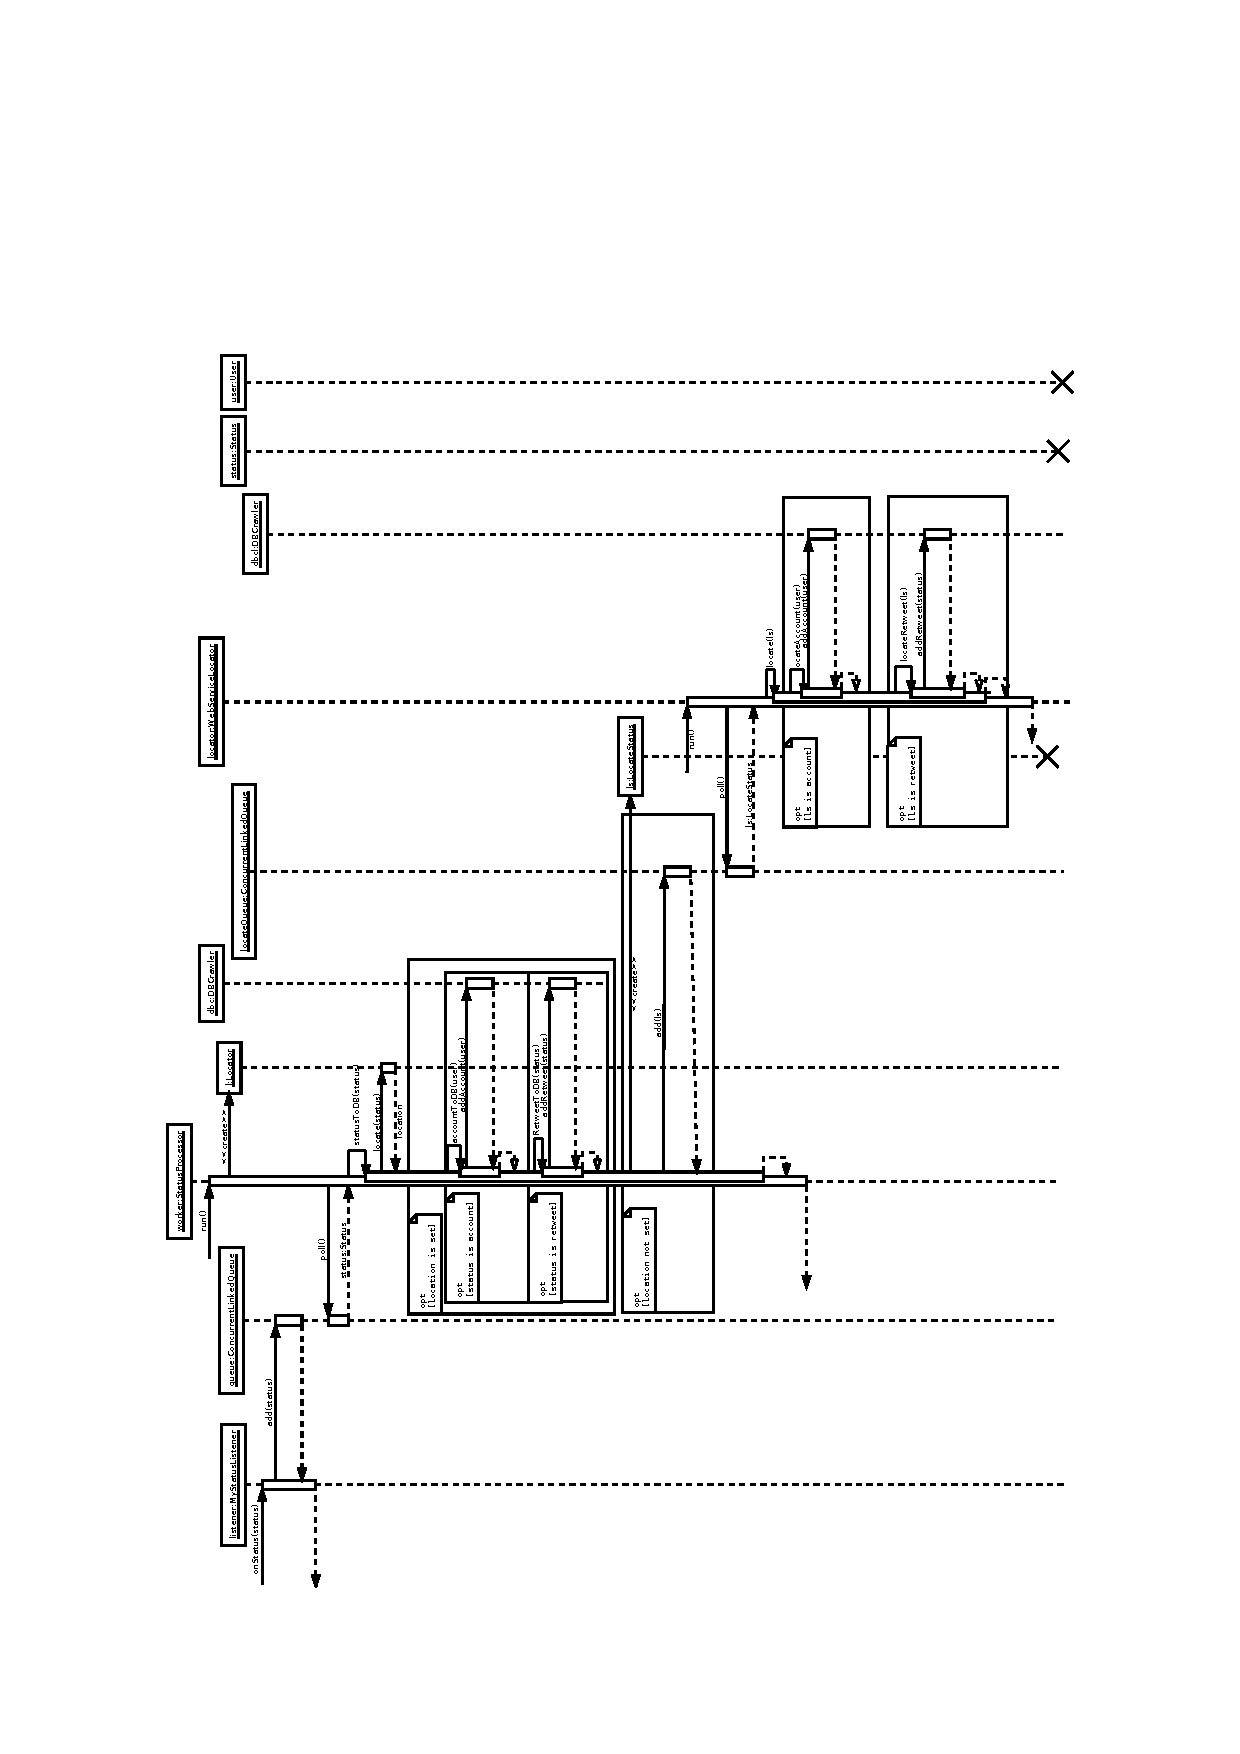
\includegraphics[width=\textwidth,height=\textheight,keepaspectratio=true]{dia/crawler_process_sequence}
	\caption{Sequenzdiagramm zur Verarbeitung der Daten durch den Crawler}
	\label{fig:Crawler}
\end{figure}

Neben dem 'Crawler' wurde auch der 'Locator' bzw. das Paket 'locate' etwas umstrukturiert, er besteht nun aus zwei (Haupt-)Klassen, welche einmal die Anfragen mittels Hashtabelle und einmal die Anfragen an den Webservice kapseln, sowie einer weiteren (Hilfs-)Klasse. Diese sind im folgenden Klassendiagramm dargestellt.
 \begin{figure}[H]
 	\centering
 	\includegraphics[width=\textwidth,height=\textheight,keepaspectratio=true]{dia/Locator}
 	\caption{Klassendiagramm locate}
 	\label{fig:locate}
 \end{figure}

\section{Änderungen am Kategorisierer}
Im folgenden Sequenzdiagramm ist der neue Ablauf des Kategorisierers dargestellt:
\begin{figure}[H]
	\centering
	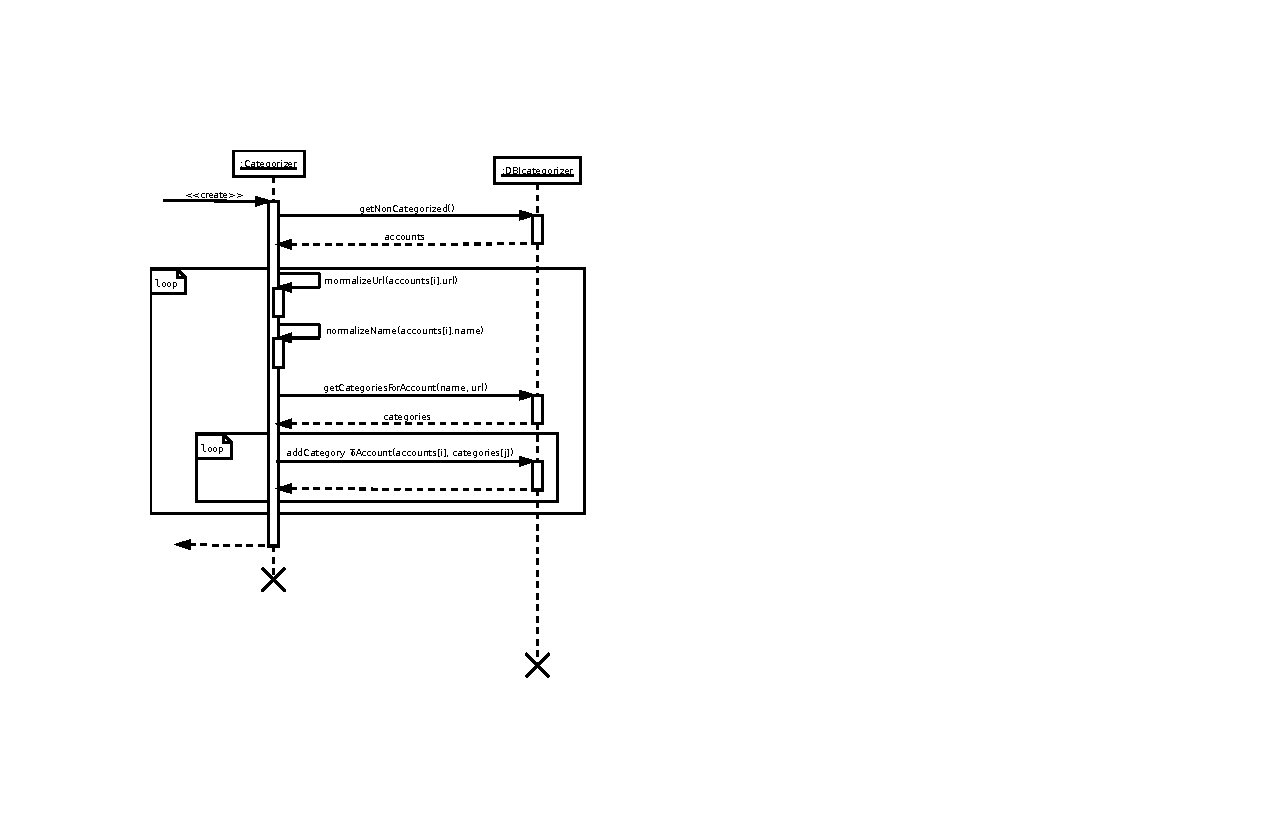
\includegraphics[width=\textwidth,height=\textheight,keepaspectratio=true]{dia/categorizerSequence}
	\caption{Sequenzdiagramm Crawler}
	\label{fig:Crawler}
\end{figure}
Gegenüber dem Entwurf sind die Methode \lstinline{normalizeUrl()} und \lstinline{normalizeName()} hinzugekommen.
\begin{itemize}
	\item \lstinline{normalizeUrl()} arbeitet mit der vom Twitteraccount angebenen URL. Es werden das Slash ("`/"') am Ende sowie Präfixe der Form \url{http://}, \url{https://} und/oder \url{www.} entfernt.
	\item \lstinline{normalizeName()} ersetzt Leerzeichen sowie Unterstriche im Benutzernamen durch ```\%'''. Diese sind das Wildcard-Zeichen in MySQL. Der so resultierende String wird zur Erhöhung der Trefferzahl in den URLs der \lstinline{page} Tabelle gesucht. Diese enthält alle URLs der DMOZ-Datenbank.
\end{itemize}
Auf diese Weise konnten bislang über 5000 Accounts kategorisiert werden.

\section{Änderungen an der GUI}
An der GUI wurden einige Änderungen zum Entwurf vorgenommen, dies lag u.A. an einer Vielzahl von Details, welche während der Entwurfsphase noch nicht bekannt waren oder bewusst auf die konkrete Implementierung verschoben wurden. 
Die Grobstruktur des Entwurfs blieb jedoch erhalten, wie das folgende Paketdiagramm (\ref{fig:GUI}) zeigt.
\begin{figure}[h!]
	\centering
	\includegraphics[width=\textwidth,height=\textheight,keepaspectratio=true]{dia/GUIPackage}
	\caption{Paketdiagramm der GUI}
	\label{fig:GUI}
\end{figure}

Eine wichtige Änderung in Bezug auf das Gesamtpaket 'gui' ist, dass es sich bei den 'View' - Klassen, welche die Darstellung der grafischen Komponenten beinhalten, um FXML Dateien handelt. FXML ist eine auf der  XML basierende Sprache, um grafische Elemente in JavaFX zu beschreiben. Dies war im Entwurf so nicht vermerkt, allerdings implizit angedacht. Die im Entwurf beabsichtigte Idee der Trennung von Darstellung und Programmlogik wird dadurch erfüllt, da die FXML-Dateien keinerlei Programmlogik enthalten. Desweiteren existiert in jedem Unterpaket von 'gui' nicht nur eine FXML-Datei mit Darstellungslogik, sondern u.U. mehrere, da so teilweise größere grafische Komponenten in einzelne FXML-Dateien gekapselt werden können.
	
Allgemein gilt, dass im Folgenden nur "`wichtige"' Änderungen dokumentiert sind.

\subsection{Änderungen im Paket gui}
Hier sollen die Änderungen beschrieben werden, die in Klassen vorgenommen wurden, welche unmittelbar im Paket "`gui"' angesiedelt sind.
\begin{itemize}
	\item \lstinline{GUIController}
	\quad 
	In der Hauptkontroller-Klasse sind einige Methoden hinzugekommen. Größtenteils waren diese im Entwurf schon angedacht nur noch nicht hinreichend konkret geplant worden. Die Änderungen im GUIController werden ausführlicher als für den Rest der (Unter-)Pakete besprochen, da es sich um die zentrale Klasse der GUI handelt.
	\begin{description}
		\item[getAccount(int)] liefert Account von DB zurück.
		\item[close()] beendet Programm.
		\item[addUserToWatch(twitter4j.User, int)] fügt Twitter-Account zur Datenbank hinzu.
		\item[getCategory(int)] liefert Kategorie von Datenbank
		\item[getCategory(String)] liefert Kategorie von Datenbank (nach Zeichenkette im Namen)
		\item[getCategoryRoot(int\text{[]})] baut Baum aus Kategorie-Items auf
		\item[getSummedData()] liefert alle Daten von Datenbank zu einer Suchanfrage
		\item[getDataByAccount()] liefert Daten aufbereitet nach Account
		\item[getDisplayValueProperty()] "`Berechnungsformel"' liefert relativen Wert zum Einfärben der Karte
		\item[getLocations()] liefert Orte von DB zurück
		\item[getMapDatailInformation()] liefert Detailinformationen zu Orten, auf welche geklickt wird
		\item[getSelectedAccounts()] liefert in Query ausgwählte Accounts
		\item[getSelectedCategories()] lieft in Query ausgewählte Kategorien
		\item[getSelectedLocations()] liefert in Query auswählte Orte
		\item[isConnected()] indiziert ob Verbindung zu DB besteht
		\item[isReady()]
		\item[main()] startet Programm
		\item[setCategory(int, int)] fügt Kategorie zu DB hinzu
		\item[setMapDetailInformation(MyDataEntry)] setzt Detailinformationen zu Orten, auf welche geklickt wird
		\item[setSelectedAccount(int, boolean)] fügt Account zu Query hinzu
		\item[setSelectedCategory(int, boolean)] fügt Kategorie zu Query hinzu
		\item[setSelectedLocation(int, boolean)] fügt Ort zu Query hinzu
	\end{description}
	\item \lstinline{SelectionHashList}
	\quad
	Diese neu hinzugekommene Klasse stellt  eine Ergänzung zum Entwurf dar, welche aus Gründen der Effizienz gewählt wurde. Mit implemtiert wird eine Hashstruktur, über die mittels Getter- und Settermethoden entschieden werden kann, ob eine Kategorie oder ein Account für ein Query an die Datenbank ausgewählt ist, bzw. diese zu einem Query hinzuzufügen.
	\item \lstinline{Labels}
	\quad
	\item \lstinline{RunnableParameter}
	\quad 
	Diese Klasse enthält zentral alle Beschriftungen, welche in der GUI verwendet werden.
	Neu hinzugekommene Klasse, die das Interface 'Runnable' so implementiert, dass dem Runnable ein Parameterübergeben werden kann.
	\item \lstinline{InfoRunnable}
	\quad
	Zusammen mit der gerade geschriebenen Klasse, wird mit der neu hinzugekommenen InfoRunnable ein Thread gestartet, der Nachrichten wie 'Verbinde mit Datenbank ...', 'Lade Daten' für eine begrenzte Zeit anzeigt.	
	Die folgende Grafik zeigt das Klassendiagramm des 'GUIControllers' zusammen mit verwandten Klassen. Allerdings sind die Klassen nicht mit all ihren Methoden und Attributen aufgeführt.
	\begin{figure}[H]
		\centering
		\includegraphics[width=\textwidth,height=\textheight,keepaspectratio=true]{dia/GUIKlassendiagramm}
		\caption{Klassendiagramm der GUI}
		\label{fig:GUI}
	\end{figure}
\end{itemize}

Im Folgenden werden die Änderungen in den Subpaketen von "`gui"' beschrieben.

\subsection{databaseOpts}
In diesem Paket wurde, wie oben vermerkt, die FXML-Datei für den grafischen Inhalt in vier separate FXML Dateien aufgeteilt, um die Lesbarkeit und Übersichtlichkeit zu erhöhen.


Weiter wurden in 'DatabaseOptController' einige Methoden und innere Klassen hinzugefügt:
\begin{itemize}
	\item \lstinline{DatabaseOptController}
	\quad
	\begin{description}
		\item[intialize]
		\quad
		Diese Methode wird aufgerufen, wenn die GUI gestartet wird. Hier werden alle grafischen Elemente mit den jeweiligen EventHandler verknüpft.
	
			\item[MyAcctionEventHandler] Innere Klasse, in ihr werden alle 'ActionEvent' behandelt. 
			\item[MyLocEventHandler] Innere Klasse, um 'Events' zu behandeln.
			\item[MyAccEventHandler] Innere Klasse, um 'Events' zu behandeln.
			\item[MyCatEventHandler] Innere Klasse, um 'Events' zu behandeln.
		\end{description}
\end{itemize}
	
Desweiteren wurden einige private Hilfsmethoden hinzugefügt, die beispielsweise einen Baum aus Kategorien aufbauen.

\subsection{table}
Diese Paket blieb relativ unverändert, lediglich die Hilfsklasse "`InternAccount"' ist aus Gründen der Effizienzsteigerung hinzugekommen.
		
\subsection{standardMap}
In diesem Paket ergaben sich einige Änderungen. Diese waren durch die relative Inkompatibilität des verwendeten Map-Frameworks "`unfolding"' mit "`JavaFX"'. Daher musste die Klasse "`StandardMapDialog"' als "`Swing-Adapter'" hinzugefügt werden. Weiterhin entschieden wir uns, sowohl  die "`StandardMap'" als auch die "`DateMap'" zu implementieren. Die "`StandardMap'" visualisiert alle vorhandenen Daten, in der "`DateMap'" können Anfangs - und Endpunkt der betrachteten Daten gewählt werden. Da die "`StandardMap'" somit einen Spezialfall der "`DateMap'" darstellt, haben wir uns entschieden, beide Pakete unter dem Namen "`StandardMap'" zu verschmelzen. Durch diese Entscheidung musste nur die "`update'" Methode geringfügig verändert werden.
\begin{itemize}
	\item \lstinline{StandardMapDialog}
	\quad
	Diese Klasse erbt von JFrame einem  Swing-Typ, da nur in Swing das verwendete Map-Framework fehlerfrei dargestellt werden kann. Sie enthält unter anderem eine Referenz auf den "`GUIController"' und auf eine Instanz von "`MyUnfoldingMap"'.
	\begin{description}
		\item[update()] diese Methode aktualisiert die auf der Karte dargestellten Daten. Die Daten werden vom "`GUIController"' bezogen und an die eigentliche Karte in "`MyUnfoldingMap"' weitergereicht. Start und Endzeitpunkt werden gesetzt, falls alle bisher gesammelten Daten in die Berechnung mit einfließen sollen, wird der Startzeitpunkt auf einen Zeitpunkt vor Beginn des Mitlesens des Twitter-Streams gesetzt.
	\end{description}
\end{itemize}
		
\subsection{csvExport}
Diese Paket war im Entwurf noch nicht berücksichtigt, da die hier realisierte Funktionalität optional war.
\subsection{unfolding} 
Die Klasse "`MyUnfoldingMap'" wurde als Singleton implementiert, da für alle bisherigen (und evtl. noch hinzukommenden) Kartendarstellungen nur eine zugrunde liegende Instanz der eigentlichen Karte benötigt wird. Diese wird jeweils aktualisiert.
\begin{description}
	\item \lstinline{MyUnfoldingMap}
	\begin{description}
			\item[getSingleton()] liefert eine Instanz der Klasse zurück
			\item[mouseClicked(MouseEvent)] Methode berechnet zu jedem Klick auf die Karte, das angeklickte Land und liefert Informationen zum jeweiligen Retweet-Verhalten.
	\end{description}
\end{description}
	